\documentclass[journal]{IEEEtran}
\usepackage{amsmath,amssymb}
\usepackage{graphicx}
\usepackage{booktabs}
\usepackage{xcolor}
\usepackage{cite}
\usepackage{tikz}
\usetikzlibrary{angles, quotes, decorations.pathreplacing, shapes.geometric, arrows.meta, positioning, backgrounds, fit}
\usepackage[hidelinks]{hyperref}

% results still to fly or to be measured: red, so none survives into a submission unnoticed
\newcommand{\placeholder}[1]{\textcolor{red}{[#1]}}
\definecolor{RED}{rgb}{1,0,0}   % IEEEtran upper-cases running heads, \textcolor{red} included

\begin{document}

\title{In-Flight Reconfiguration of a Cable-Suspended Ring Carried by a Team of Quadrotors}

\author{Wesley~Donald, Mitchell~Torok, and~Mohammad~Deghat%
\thanks{The authors are with the School of Mechanical and Manufacturing Engineering, UNSW Sydney, Australia
\placeholder{affiliations and e-mail addresses to confirm}.}}

\markboth{IEEE Robotics and Automation Letters. Preprint version, 2026}%
{Donald \MakeLowercase{\textit{et al.}}: In-Flight Reconfiguration of a Cable-Suspended Ring}

\maketitle

\begin{abstract}
Teams of quadrotors carrying a cable-suspended payload usually keep a fixed composition throughout a
flight. We show that model predictive control lets such a team drop and re-add carriers in flight. A centralised
planner solves an optimal control problem over a 0.86\,kg ring and every carrier's cable, and per-carrier trackers
follow its plan on unmodified Betaflight quadrotors. Because the attachment geometry is a runtime parameter, a change
of team is a switch to a pre-built problem of the new size, warm-started from the measured state. Three
reconfigurations are handled: an unannounced release, detected when the leaver's rod reads
longer than itself; the rejoin of a departed carrier, welded within 1.5\,cm of its own plate and blended into the
load over 10\,s with the path held; and the attach of a newcomer flown by another controller, admitted only after
magnet contact and a motion-capture proof of co-motion. It is validated in a digital twin
built from the rig's thrust map and geometry, and on a motion-capture rig, where an unannounced release is detected
in 0.42\,s and the ring's tilt peaks at 6.5$^\circ$, back within its band 1.8\,s later. In the twin a team of eight
carriers drops to four and rejoins all four, and on a 0.4\,m/s line our planner's path error is about half that of the
dissipative network of Quan et al., whose point-load model leaves a rim-hung ring's yaw undamped.
\end{abstract}

\begin{IEEEkeywords}
Aerial systems: mechanics and control, multi-robot systems, cooperative manipulation, model predictive control,
cable-suspended payload.
\end{IEEEkeywords}

\section{Introduction}
\label{sec:intro}

Several quadrotors sharing a payload on cables can lift what none of them could carry alone, and spread the load so
that each flies with margin \cite{olleroPresentFutureAerial2022, estevezReviewAerialTransportation2024}. Such a team
is almost always treated as fixed: the carriers are attached on the ground, take off together and land together. A
team that could change in the air would be more useful and more robust. A carrier with a low battery or a fault could
leave and come back; a fresh carrier could join to take up a heavier load or relieve another; and a carrier that is
lost without warning, a released magnet or a failed motor, need not bring the payload down with it. This letter
asks what a controller needs to let a team carrying a cable-suspended payload lose and gain carriers in flight.

\emph{Cooperative cable transport.} The statics of a rigid payload hung from several cables, and the internal forces
the team may choose freely, are well understood \cite{michael2011cooperative, tognon2018internal,
gabellieri2023equilibria}. Controllers range from decentralised schemes that need no communication between carriers
\cite{tognon2018internal, gabellieri2023force, klausen2020cooperative} through geometric and leader--follower designs
\cite{lee2018geometric, loianno2018cooperative} to the passivity-based dissipative network of Quan et
al.~\cite{quan2025swarm}. Model predictive control (MPC) suits the problem because cable tensions are bounded and
the payload's motion couples every carrier: nonlinear MPC of the full payload pose \cite{sunNonlinearMPCFullPose2023,
liNonlinearModelPredictive2023}, kinodynamic planning for the team \cite{wahbaKinodynamicMotionPlanning2024}, and
distributed formulations \cite{decarliDistributedNMPCCooperative, distributedNMPC} all fly a team of a fixed size.

\emph{Reconfiguration and attach.} Plug-and-play MPC adds and removes subsystems from a distributed controller
\cite{riverso2013plug, zeilinger2013plug, aboudonia2022reconfigurable, saccani2023model}, but for networks of
loosely coupled plants, not for carriers that share one payload. Modular aerial robots dock and undock in flight
\cite{saldana2018modquad, sugihara2023trady, sugihara2026legion}, and magnetic grippers let a multirotor pick up and
release objects \cite{gawel2017magnetic, miyazaki2018airborne}. Fault-tolerant cooperative transport keeps a payload
up after a carrier fails \cite{liang2021fault, farrasFaultTolerantControlMultiQuadcopter2024}. We know of no work
in which a team carrying a cable-suspended payload both loses carriers without warning and admits carriers that join
in the air, nor of one flown on hardware.

The working hypothesis of this letter is that a centralised optimal control problem suits a change of team because
the planner solves for the force distribution of the team it actually has in the first tick after the event,
instead of leaving the survivors to find it from the motion that follows. The contributions are:
\begin{itemize}
  \item a cooperative MPC for a cable-suspended ring whose attachment geometry is a runtime parameter, so that a
  change of team is a switch to a pre-built problem of the new size, warm-started from the measured state
  (Section~\ref{sec:method});
  \item detection of an unannounced release from motion capture alone, a drop rule from the support margin of the
  survivors, and the rejoin of a departed carrier to its own plate in flight (Sections~\ref{sec:reconfig}
  and~\ref{sec:rejoin});
  \item the attach of a newcomer flown by another team's controller, admitted only on a motion-capture proof that its
  magnet moves with the ring;
  \item validation in a digital twin built from the rig's identified thrust map and geometry and on a
  motion-capture rig with unmodified Betaflight quadrotors, with a scalability study and a comparison against our
  port of Quan et al.'s method \cite{quan2025swarm} (Sections~\ref{sec:res_reconfig}--\ref{sec:res_compare}).
\end{itemize}

\section{System}
\label{sec:system}

\emph{Payload.} The payload is a ring of mass $m_L = 0.86$\,kg carrying twelve magnet plates every $30^\circ$ at
radius $r = 0.225$\,m (Fig.~\ref{fig:geometry}). Plates are numbered clockwise from the ring's $+x$ axis seen from
above. A carrier hangs from a plate on a link of length $l_i$, 1\,m in the results here, whose lower end holds an
electromagnet switched over the carrier's radio channel; the links fly at about $60^\circ$ from horizontal. The
magnet catches only on contact with its plate, so a release needs no mechanism beyond switching it off.

\emph{Rig.} The carriers are 0.55\,kg quadrotors on unmodified Betaflight flight controllers, whose inner rate loop
is kept; our trackers send a collective throttle and three body-rate commands over the radio link. A motion-capture
system measures the pose of every quadrotor, the ring and the links' lower ends in a $6\times6\times4$\,m cage, and a
position limit of $\pm1.75$\,m lands the fleet if any quadrotor leaves it. Thrust is affine in throttle, with an
offset that grows with the carried mass and falls with battery voltage; the map was identified on the rig from free
hovers with hung masses over the battery's range.

\emph{Digital twin.} A Gazebo \cite{koenig2004gazebo} model under ROS~2 \cite{macenski2022ros2} reproduces the
rig: the same masses, geometry, identified thrust map and rate-loop model, the motion-capture velocity filter, and
the same planner, trackers and safety logic, launched unchanged against simulated topics. The twin models every link
as rigid, whereas the rig's tethers can go slack; slack-cable effects and the rig's unmodelled aerodynamics are
therefore its honest limit, and the rig flights are the check on it.

% fig_geometry.tex -- M3: payload and rod geometry (TikZ). Dimensions from the rig (30 Sep 2026):
% plates at r 0.225 m on a 500 mm ring, 12 plates every 30 deg, rod 0.55 m, pivot 4 cm below the UAV centre.
% 17 Oct: plates numbered clockwise from +x seen from above (angle = 30 x plate, Wesley 14 Oct); the side view at
% the planned elevation of 60 deg (since 7 Oct). Drawn to scale (1 m = 9 cm).
\begin{figure*}[t]
\centering
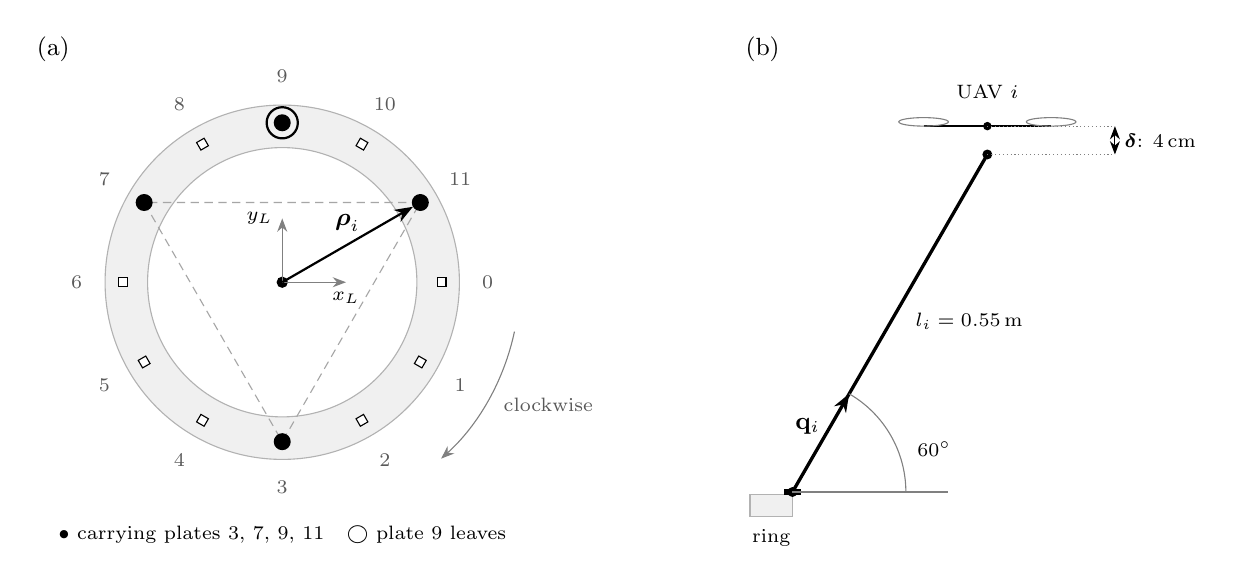
\begin{tikzpicture}[x=9cm, y=9cm, >=Stealth, font=\small]
  % ---------------- (a) top view ----------------
  \begin{scope}
    \fill[gray!12] (0,0) circle (0.25);
    \fill[white] (0,0) circle (0.19);
    \draw[gray!60, thin] (0,0) circle (0.25) (0,0) circle (0.19);
    % the even triangle left after plate 9 leaves
    \draw[densely dashed, gray!70] (30:0.225) -- (150:0.225) -- (270:0.225) -- cycle;
    % plates, numbered clockwise from +x
    \foreach \k in {0,...,11} {
      \pgfmathsetmacro{\a}{-30*\k}
      \node[draw, fill=white, minimum size=0.11cm, inner sep=0pt, rotate=\a] at (\a:0.225) {};
      \node[font=\scriptsize, text=gray!70!black] at (\a:0.29) {\k};
    }
    % the four carrying plates: 3, 7, 9 and 11
    \foreach \k in {3,7,9,11} { \fill[black] (-30*\k:0.225) circle (0.012); }
    \draw[thick, black] (-270:0.225) circle (0.022);
    % centre, axes, rho
    \fill (0,0) circle (0.008);
    \draw[->, thin, gray] (0,0) -- (0.09,0) node[below, font=\scriptsize, text=black] {$x_L$};
    \draw[->, thin, gray] (0,0) -- (0,0.09) node[left, font=\scriptsize, text=black] {$y_L$};
    \draw[->, thick] (0,0) -- (30:0.213) node[pos=0.62, above left, inner sep=1pt] {$\boldsymbol{\rho}_i$};
    \draw[->, gray] (-12:0.335) arc (-12:-48:0.335);
    \node[font=\scriptsize, text=gray!70!black, anchor=west] at (-30:0.345) {clockwise};
    \node[font=\scriptsize, align=left, anchor=north] at (0,-0.33) {$\bullet$ carrying plates 3, 7, 9, 11\quad $\bigcirc$ plate 9 leaves};
    \node[anchor=north west] at (-0.36,0.36) {(a)};
  \end{scope}
  % ---------------- (b) side view of one rod (A plate, P pivot, C UAV centre), elevation 60 deg ----------------
  \begin{scope}[shift={(0.72,-0.33)}]
    \fill[gray!12] (-0.06,0) rectangle (0.0,0.03);
    \draw[gray!60, thin] (-0.06,0) rectangle (0.0,0.03);
    \fill[black] (-0.012,0.03) rectangle (0.012,0.038);
    \coordinate (A) at (0,0.034);
    \coordinate (P) at (0.275,0.5103);
    \coordinate (C) at (0.275,0.5503);
    \draw[very thick] (A) -- (P);
    \fill (A) circle (0.007) (P) circle (0.007);
    \draw[thick] (0.185,0.5503) -- (0.365,0.5503);
    \draw[gray] (0.185,0.5563) ellipse (0.035 and 0.006) (0.365,0.5563) ellipse (0.035 and 0.006);
    \fill (C) circle (0.006);
    \draw[->, thick] (A) -- (0.08,0.1726) node[pos=0.55, above left, inner sep=1pt] {$\mathbf{q}_i$};
    \draw[gray] (0.16,0.034) arc (0:60:0.16);
    \draw[gray, thin] (A) -- (0.22,0.034);
    \node[font=\scriptsize] at (0.20,0.095) {60$^\circ$};
    \node[font=\scriptsize, anchor=north west] at (0.16,0.30) {$l_i = 0.55$\,m};
    \draw[gray, thin, densely dotted] (P) -- (0.455,0.5103) (C) -- (0.455,0.5503);
    \draw[<->, thin] (0.455,0.5103) -- (0.455,0.5503) node[midway, right, font=\scriptsize] {$\boldsymbol{\delta}$: 4\,cm};
    \node[font=\scriptsize, anchor=north] at (-0.03,-0.005) {ring};
    \node[font=\scriptsize, anchor=south] at (0.275,0.575) {UAV $i$};
    \node[anchor=north west] at (-0.08,0.69) {(b)};
  \end{scope}
\end{tikzpicture}
\caption[Payload and rod geometry]{Payload and rod geometry, to scale. (a) Top view of the 0.86\,kg ring
with its twelve magnet plates at a radius of 0.225\,m, numbered clockwise from the $x_L$ axis seen from above, so
that plate $k$ sits $30k$ degrees clockwise from $x_L$. The four-UAV layout uses plates 3, 7, 9 and 11; when the
UAV on plate 9 leaves, the three on plates 3, 7 and 11 form an even triangle (dashed), under which the ring hangs
level. (b) Side view of one rod at the planned elevation of 60$^\circ$: the rod direction $\mathbf{q}_i$ points
from the plate to the UAV, and the rod pivots $\boldsymbol{\delta}$ = 4\,cm below the UAV's centre. Rig dimensions
(0.55\,m rods); the twin results use 1\,m cables.}
\label{fig:geometry}
\end{figure*}

\section{Method}
\label{sec:method}

The controller is a two-level cascade. A centralised planner plans the motion of the ring and of every link over a
horizon; a tracking MPC on each carrier follows that carrier's share of the plan. A change of team is handled
inside the planner, by changing the problem it solves.

\subsection{Cooperative planner and trackers}
\label{sec:planner}

The planner's model is the ring as a rigid body, pose $(\mathbf{p}_L, \mathbf{q}_L)$ and twist $(\mathbf{v}_L,
\boldsymbol{\omega}_L)$, with each of the $N$ carriers reduced to a link of length $l_i$ attached at the plate
point $\boldsymbol{\rho}_i$ in the ring frame, with unit direction $\mathbf{q}_i$ and tension $\lambda_i$. The
carrier positions follow kinematically, $\mathbf{p}_i = \mathbf{p}_L + R(\mathbf{q}_L)\boldsymbol{\rho}_i -
l_i\mathbf{q}_i$, and the thrust each must produce follows from its link's acceleration and tension. At every
tick the planner solves
\begin{equation}
\begin{aligned}
  \min_{\mathbf{x}_{0:N_h},\,\mathbf{u}_{0:N_h-1}} \;& \sum_{k=0}^{N_h-1} \|\mathbf{y}_k - \mathbf{y}_k^{\mathrm{ref}}\|_W^2
    + \|\mathbf{y}_{N_h} - \mathbf{y}_{N_h}^{\mathrm{ref}}\|_{W_{N_h}}^2 \\
  \text{s.t.}\;& \mathbf{x}_{k+1} = \mathbf{F}(\mathbf{x}_k, \mathbf{u}_k;\, \{\boldsymbol{\rho}_i, l_i\}, \mathbf{d}),
    \quad C_0\mathbf{x}_0 = C_0\hat{\mathbf{x}}(t), \\
  & \lambda_{\min} \le \lambda_{i,k} \le \lambda_{\max}, \quad f_{\min} \le \|\mathbf{f}_{i,k}\| \le f_{\max},
\end{aligned}
\label{eq:ocp}
\end{equation}
where the output $\mathbf{y}$ stacks the ring's position, velocity, attitude error and rate, the link directions,
tensions and rates, and the inputs; $\mathbf{f}_{i,k}$ is carrier $i$'s planned thrust, its bounds softened with
slack. The horizon has $N_h = 20$ nodes over 2\,s, so a node is the 100\,ms planner tick. The constraint on node~0
pins only what motion capture measures, the ring's pose and twist and the link directions; the tensions and link
rates are left free and warm-started from the previous solution. A lumped force $\mathbf{d}$ on the ring, formed
from the integral of its position error in steady flight, removes steady offsets through the model
\cite{pannocchia2003disturbance, maeder2009linear}. The references follow from the ring's trajectory by flatness,
with the nominal formation tilted along the effective gravity and the tensions scaled with it.

Problem~\eqref{eq:ocp} is solved with acados \cite{verschueren2022acados} in a real-time iteration scheme
\cite{diehl2002rti}: one Gauss--Newton SQP iteration per tick, warm-started, with HPIPM \cite{frison2020hpipm}
solving the QP. On the rig no new iteration starts after 60\,ms of the tick, and a plan not ready by then is replaced
by the previous one shifted by a node.

Each carrier's tracker is an MPC on a 17-state model in which the four stick commands are states and their rates the
inputs, with the flight controller's rate loop modelled as first order and the identified affine thrust map. It
solves every 20\,ms over the same 2\,s horizon, following the planner's position, velocity and thrust direction. The
link's pull enters its model as a known parameter along the horizon: the planned pull, shifted by the difference
between the pull measured from motion capture and the planned one at the first node, so that the tracker anticipates
the link's force rather than reacting to it.

\subsection{Reconfiguration: release and drop}
\label{sec:reconfig}

Two properties of \eqref{eq:ocp} make an in-flight change of team possible. The plate points
$\boldsymbol{\rho}_i$ and link lengths $l_i$ are runtime parameters, so only the team size fixes the problem's
dimensions, and one solver per size, built in advance and primed on the measured state, covers any layout. And the
survivors keep their own plates: the nominal tensions come from a moment balance at the actual plate points, so the
ring's reference stays level without re-spacing the team.

\emph{Detection.} A release the planner is told of is a DETACH command, which switches the leaver's magnet off and
resizes on the same tick. An unannounced release is detected from the link alone. A rigid link on its plate cannot
measure longer than itself, so when the leaver's link, measured by motion capture between the carrier's pivot and
its plate point, reads more than 6\,cm over its length for two consecutive ticks, the planner removes that carrier.
No force sensor and no message from the leaver are needed.

\emph{Resize.} At the event the planner swaps to the solver for $N-1$ carriers, sets the survivors' plate points and
link lengths, and warm-starts it from the measured state with the tensions and link directions free at node~0. The
first solve redistributes the load; there is no separate hand-off phase. With three survivors the vertical shares
are fixed by statics: each is the ring's weight times the barycentric coordinate of its centre in the survivors'
triangle, and a level ring exists only while the centre lies inside the polygon of the plates
\cite{michael2011cooperative}. For plates on a circle of radius $r$, with $g_{\max}$ the survivors' largest angular
gap, the support margin
\begin{equation}
  m = r\cos(g_{\max}/2)
  \label{eq:margin}
\end{equation}
is the distance from the centre to the nearest edge. Losing one of four evenly spaced carriers puts the centre on an
edge, so the four-carrier layout uses plates 3, 7, 9 and 11, where losing plate 9 leaves an even triangle with a
112\,mm margin.

\emph{Drop rule.} A loss that leaves fewer survivors than the configured minimum (three by default), or a ring tilt
above $30^\circ$, drops the ring: every magnet is switched off and every carrier lands. Release chains that continue
below three carriers fly on while the survivors' largest gap is at most $200^\circ$, which keeps a T and an opposite
pair. The freed carrier steps out radially, clear of the ring, and lands and disarms alone while the survivors carry
on.

\subsection{Rejoin of a departed carrier}
\label{sec:rejoin}

A departed carrier can return to its own plate. At its release the planner records its plate point and the link's
measured length. \emph{Staging:} the carrier is held on its plate's bearing 0.3\,m beyond the formation's reach,
the point moving and turning with the planned ring and kept inside the position limit. \emph{Approach:} on the
rejoin command, given only while the ring holds its path, the carrier descends at 0.1\,m/s so that its link's
lower end lands on the plate point of the measured ring, with a feedback loop on the measured end correcting the
end's height. \emph{Weld:} the magnet is switched on once the end has stayed within 1.5\,cm of its plate point on
every sample over 0.3\,s (at least eight samples) at under 2\,cm/s; the joint must then report attached, or the
carrier is let go and backs out to staging. \emph{Fold-in:} the planner grows to $N+1$ with the plate point and the
link re-measured from pivot to plate; the rejoiner is seeded at 0.1\,N and every tension is blended to the balanced
split over 10\,s, with its link feedforward ramped over 1.5\,s and the ring's path held throughout, as a dock blends
thrust across a switch \cite{sugihara2023trady}. Through the blend the rejoiner's height reference is capped at the
weld height, so that it cannot lift its plate and tilt the ring before it carries its share, and it counts as absent
for the drop rule. LAND or a drop sends every staged or rejoining carrier up, out along its bearing and down alone.

\subsection{Attach of a newcomer}
\label{sec:attach}

A newcomer is flown by another team's controller down to contact; its magnet catches only there. Our side admits it
from motion capture alone, with its magnet tip expressed in the plate's frame. A \emph{contact} is the tip within
24\,mm of the plate point and close to the plate's face, nearly still for 0.3\,s. A contact is only a candidate, since
a tip resting on a plate and a caught magnet look alike, so the catch is \emph{confirmed} by co-motion: after the
newcomer's small lift, the tip has stayed within 6\,mm of its contact point while the plate moved with it, on a taut
tether. Only then do our trackers take the newcomer over and the planner grows to $N+1$ with the recorded plate
point, the newcomer seeded at 0.1\,N and blended as in Section~\ref{sec:rejoin}. A newcomer not confirmed in time is
taken back: our tracker latches onto its measured state, lifts it clear and lands it alone.

% 04_results.tex -- results half, draft 23 Oct 2026. Pending results are \placeholder{}.
\section{Results}
\label{sec:results}

We test our planner on the rig and in its simulated twin. The rig carries the 0.86\,kg ring with magnet plates every
30$^\circ$ on its rim; the twin models the same ring, the same quadrotors and the rig's thrust map and motion-capture
filter, but its cable links are rigid. Unless stated otherwise the twin flies 1\,m cables with the ring at 1.0\,m.
Bars were written before each set of runs, and a run is scored against the bars of its set only.

%-------------------------------------------------------------------------------------------------------------------
\subsection{Release and rejoin}
\label{sec:res_reconfig}

\paragraph{An unannounced release on the rig}
Four carriers hover the ring on the rig, and one of them lets go of its plate without telling the planner.
Fig.~\ref{fig:release} shows the reaction of Section~\ref{sec:reconfig}. The planner sees the released cable stretch
past its threshold 0.42\,s after the release and resizes its problem to three carriers 0.09\,s later, each survivor
then planned at about 3.2--3.3\,N. The ring's tilt peaks at 6.5$^\circ$ and is back in its band 1.8\,s after the
release (Table~\ref{tab:release}). Over all three rig releases, detection took 0.33--0.42\,s and the ring was back in
band within 1.8--3.8\,s; the slowest, with the largest tilt, left a 150$^\circ$ gap between survivors. An announced
detach, by contrast, resizes at the command but tilted the ring further, to 15.4$^\circ$. In the twin, the same
release on 1\,m cables resized after 0.37\,s with a 5.9$^\circ$ tilt peak.

\begin{figure}[t]
\centering
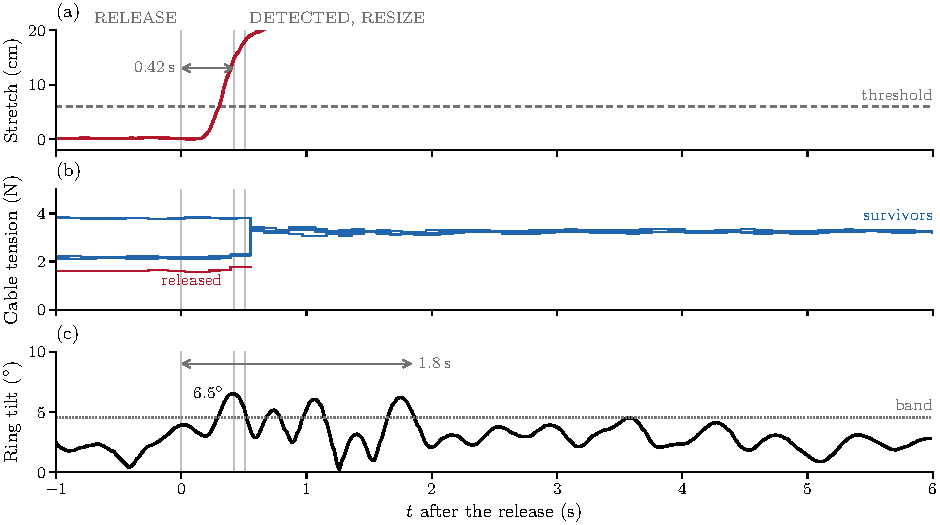
\includegraphics[width=\columnwidth]{figures/fig_release.pdf}
\caption{An unannounced release on the rig: one of four carriers (red) lets go of its plate in hover. The planner
detects the loose cable from its stretch, resizes to the three survivors (blue), and the ring's tilt (black) returns
to its band.}
\label{fig:release}
\end{figure}

\begin{table}[t]
\centering
\footnotesize
\setlength{\tabcolsep}{3pt}
\caption{Reaction to a lost carrier, four carriers in hover. Times from the release (or the command). Rig: 0.55\,m
rods; twin: 1\,m cables.}
\label{tab:release}
\begin{tabular}{lcccc}
\toprule
 & Detected & Resized & Tilt peak & Back in band \\
Case & (s) & (s) & ($^\circ$) & (s) \\
\midrule
Rig, release (Fig.~\ref{fig:release}) & 0.42 & 0.51 & 6.5 & 1.8 \\
Rig, all three releases & 0.33--0.42 & \placeholder{to measure} & 6.5--17.8 & 1.8--3.8 \\
Rig, announced detach & -- & 0 & 15.4 & 1.95 \\
Twin, release & -- & 0.37 & 5.9 & 3.4 \\
\bottomrule
\end{tabular}
\end{table}

\paragraph{A departed carrier rejoins (twin)}
A released carrier is not landed: it holds a staging point beyond its own plate and, on the operator's command,
flies back, is re-attached and is folded into the team (Section~\ref{sec:rejoin}). This is a twin result only, since
the twin's joint welds the cable wherever its end lies, while the rig's magnet catches only on contact. A rejoin is
scored in stages, each against a bar frozen before the runs: the cable's end on its plate within 30\,s; the joint
attached within 0.5\,s of that; then the fold-in, with the ring's tilt at most 5$^\circ$ from the weld to 15\,s
after it, the end within 2\,cm of its plate through the 10\,s blend, and the rejoiner's planned pull at the blend's end
within 10\,\% of its share. Table~\ref{tab:rejoin} gives the results onto a square (four carriers back from three) and
onto a T (three back from an opposite pair); Fig.~\ref{fig:rejoin} shows one rejoin onto the T.

Every rejoin welded within 1.5\,cm of its plate point, and the fold-in tilted the ring by 1.3--3.4$^\circ$. With a
steady torque leaning the T's pair about 3$^\circ$, the rejoin passed 3 of 4 runs: in one run leaning toward the
rejoin plate the ring tipped to 5.28$^\circ$ for 0.19\,s, missing the bar by 0.28$^\circ$. There the rejoiner's
height reference, held at or below its weld height through the blend to stop its rigid link lifting the T's free side,
dipped 1.1\,cm at the fold-in. The hold patches a twin artefact, a rigid link, which the rig's slack tethers do not
share. Two neighbouring checks also passed: a LAND during the rejoin's descent sends the rejoiner up, out and down
alone, 1.245\,m from the ring's centre (bar 1.2\,m), and a carrier staged through a figure-eight lap of the T stays
inside the position limit, with its attach command refused while the path moves.

\begin{table}[t]
\centering
\footnotesize
\setlength{\tabcolsep}{2.2pt}
\caption{A departed carrier rejoins its own plate (twin, hover, 1\,m cables), final code tree. Bars, frozen before
the runs, in brackets. Leaning: a steady torque leans the T's pair about 3$^\circ$. Ranges over $n$ runs.}
\label{tab:rejoin}
\begin{tabular}{lccccc}
\toprule
 & & On plate & Weld & Fold-in & End from \\
Rejoin & $n$ & after (s) & after (s) & tilt ($^\circ$) & plate (cm) \\
 & & [30] & [0.5] & [5] & [2] \\
\midrule
Square & 4 & 23.9--24.9 & 0.029--0.036 & 1.27--1.55 & 1.3--1.6 \\
T & 3 & 16.6--17.7 & 0.012--0.021 & 1.45--3.02 & 1.3--1.5 \\
T, leaning toward & 2 & 15.6--16.5 & 0.015--0.018 & 3.12--\textbf{5.28} & 1.3--1.5 \\
T, leaning away & 2 & 17.7--18.6 & 0.015--0.018 & 2.91--3.37 & 1.4--1.5 \\
\bottomrule
\end{tabular}
\end{table}

\begin{figure}[t]
\centering
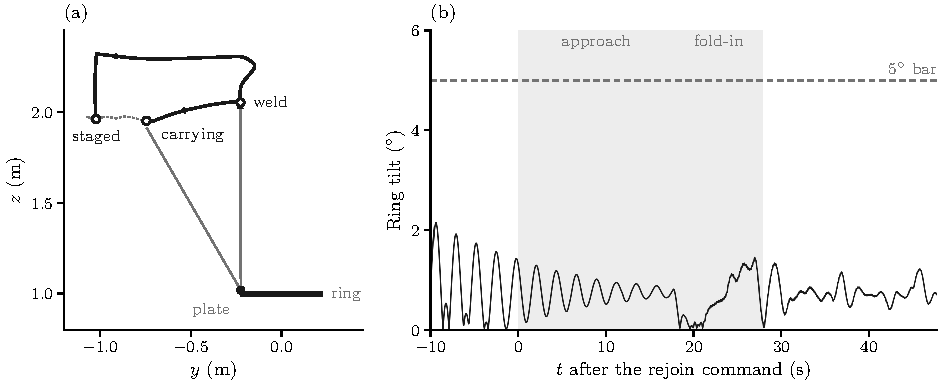
\includegraphics[width=\columnwidth]{figures/fig_rejoin.pdf}
\caption{A carrier released from the T flies back to its own plate in the twin, re-welds 17.8\,s after the rejoin
command and folds back in. (a) The rejoiner's path, side view, with its cable at the weld and folded in; (b) the
ring's tilt, peaking at 1.45$^\circ$ in the fold-in, against the 5$^\circ$ bar.}
\label{fig:rejoin}
\end{figure}

\paragraph{Eight to four and back (twin)}
Release and rejoin compose into a chain. Eight carriers at 45$^\circ$ on 1\,m cables lift a 0.9\,kg ring of radius
0.5\,m from the floor; every other carrier is released unannounced, one at a time and 15\,s apart, down to a square of four,
and the four freed carriers then rejoin one at a time back to eight (Fig.~\ref{fig:s_chain}). In both claim runs, at five
solver iterations per tick, no drop or abort fired; each release raised the ring's tilt by at most 2.9$^\circ$ with the
planner resized within 0.4\,s, and each rejoin's planner grew within 16.2--19.4\,s of its start. Back at eight, scored from
2\,s after the last rejoin's blend ends, the ring's tilt held its bar (0.95--0.99$^\circ$) but its position error, 6.4\,mm
(rms) in both runs, missed its bar of 5.7\,mm: the last fold-in leaves the ring 36\,mm off, and it returns over about 5\,s.
The world runs at about a quarter of real time here, so these runs are about the plan and the physics, not about timing
(Section~\ref{sec:res_scale}).

\begin{figure}[t]
\centering
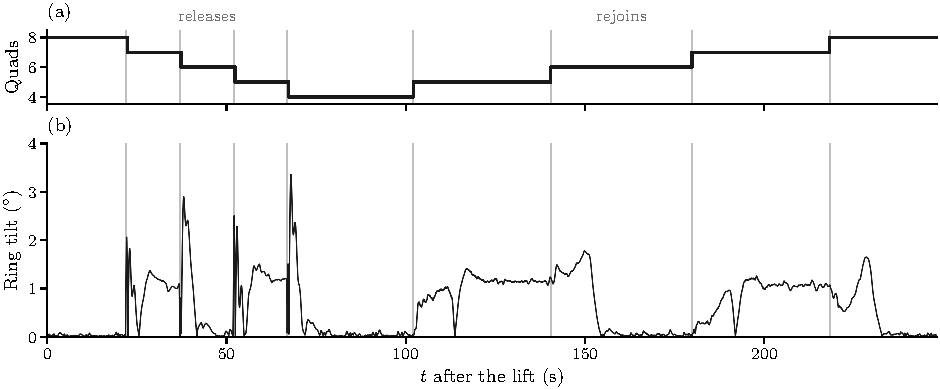
\includegraphics[width=\columnwidth]{figures/fig_s_chain.pdf}
\caption{Eight carriers take the 0.9\,kg, 0.5\,m ring through four unannounced releases down to four and four
rejoins back to eight (twin, not real time; an earlier exploratory run at one iteration a tick, the claim runs at
five described in the text). (a) The team size the planner flies; (b) the ring's tilt, peaking at 3.35$^\circ$.}
\label{fig:s_chain}
\end{figure}

\paragraph{A newcomer attaches on the rig}
\placeholder{The rig attach of a newcomer on 1\,m cables (three carriers to four with the basket): flies 29 Oct.}


\subsection{Scalability}
\label{sec:res_scale}

Our planner solves the OCP~\eqref{eq:ocp} with a fixed number of sequential-quadratic-programming (SQP) iterations
per 100\,ms tick, warm-started from the previous plan. Fewer iterations shorten the tick but leave the plan short of
convergence. We measure what that costs against the fleet size in two ways. In closed loop, the four-carrier twin
flew a hover, the figure-eight at 0.2\,m/s and an unannounced release, each from a floor start, at one iteration and
at five. Offline, each plan at one and two iterations was compared with the plan converged from the same iterate. The
bars of both checks were fixed before the runs: the dynamics residual of the plan, the error of the references the
trackers fly at the next node and the fifth, the error of the thrust feed-forward, and the cost's ratio to the
converged plan's.

In closed loop at four carriers, one iteration a tick flew as well as five in every cell. The ring's path error and
tilt stayed inside the bars set from the five-iteration runs through the lift, the path and the release, and no run
dropped, aborted or failed a solve. The plans were not converged, however: their dynamics residual peaked at the
release, under the closed loop's limit but over the offline bar.

Offline, the answer depends on the fleet. Replayed tick by tick, nine recorded flights with two to four carriers, the
rig's among them, converge by every bar at two iterations; at one iteration every rig flight breaks the residual bar.
At eight carriers on the figure-eight, with each warm start moved off the plan by about the rig's ring error, one
iteration misses every bar, two miss only the feed-forward bar (0.316 against 0.3\,m/s$^2$), and five pass all of
them (Table~\ref{tab:quality}, Fig.~\ref{fig:quality}). The iteration count must therefore grow with the fleet: two
suffice up to four carriers, while eight need five.

\begin{table}[t]
\centering
\footnotesize
\setlength{\tabcolsep}{4pt}
\caption{Plan quality at eight carriers against SQP iterations per tick: the figure-eight at 0.2\,m/s, each warm
start 1\,cm and 10\,cm/s off the plan, compared with the plan converged from the same iterate; 95th percentiles over
200 ticks. Bold: over the bar. No solve failed.}
\label{tab:quality}
\begin{tabular}{lcccc}
\toprule
Measure & Bar & 5 & 2 & 1 \\
\midrule
Cost ratio, median / 95th pct. & 1.10 / 1.50 & 1.000 / 1.001 & 1.003 / 1.010 & \textbf{miss}$^a$ \\
Dynamics residual & $10^{-3}$ & $3.2{\times}10^{-7}$ & $8.8{\times}10^{-5}$ & $\mathbf{9.3{\times}10^{-3}}$ \\
Reference, node 1 / 5 (mm) & 5 / 10 & 0.9 / 0.9 & 3.2 / 5.1 & \textbf{7.3} / \textbf{14.5} \\
Feed-forward (m/s$^2$) & 0.3 & 0.12 & \textbf{0.316} & \textbf{0.60} \\
\bottomrule
\multicolumn{5}{p{0.95\columnwidth}}{\footnotesize $^a$\,170 of 200 ticks over the residual bar, each counted as a
miss.}
\end{tabular}
\end{table}

\begin{figure}[t]
\centering
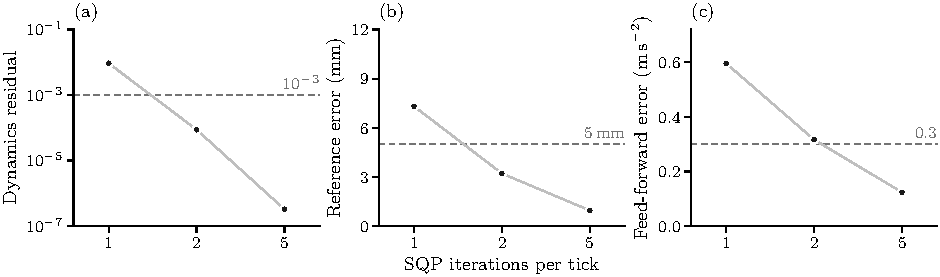
\includegraphics[width=\columnwidth]{figures/fig_s_quality_n8.pdf}
\caption{Plan quality at eight carriers against SQP iterations per tick, relative to the converged plan: the
dynamics residual, the reference error at the next node and the thrust feed-forward error (95th percentiles), with
the bars fixed before the runs. One iteration misses every bar, two miss only the feed-forward bar, five pass.}
\label{fig:quality}
\end{figure}

What this means for real time is set by the slowest tick. On the rig laptop, a bench calibrated against the rig's own
flights gives the largest team our planner flies within the 100\,ms period at five iterations as
\placeholder{$N_{\max}$ on the rig laptop at 5 iterations, from the bench with the speed-ups and the pivot}. At
eight carriers the plan must be read at five iterations, which the rig laptop cannot run in real time; the
eight-carrier results are therefore the twin's, with its clock slowed, and say nothing about real time. In the twin,
eight carriers lifted a larger ring from the floor and carried it through four unannounced releases, in opposite
pairs, to a square of four and back to eight by rejoins (Fig.~\ref{fig:s_chain}), with the ring's tilt peaking at a few
degrees and no drop. \placeholder{the eight-carrier claim runs at 5 iterations, hover and $8 \to 4 \to 8$, two each:
ring position error and tilt peak with the team back at eight, scored from 2\,s after the last rejoin's blend ends;
release tilt peak; achieved real-time factor and late ticks}.

\subsection{Comparison with a dissipative network}
\label{sec:res_compare}

A virtual spring--damper network~\cite{quan2025swarm} is the natural comparison for a team that changes in flight: a
member leaving or joining needs no new solver. We ported Quan et al.'s dissipative network to our system and flew it
against our planner in the twin. Four carriers sit on plates 0, 3, 6 and 9, with 1\,m cables and the ring at 1.0\,m.
The cases are a hover and a 0.9\,m line out and back. Both arms are our planner up to the hand-over (creep, lift and a
5\,s hover). After it, our arm keeps the planner of Sec.~\ref{sec:method} and its trackers. The network instead drives
the trackers' velocity loop with no integral per UAV. The comparison is therefore between the two methods as flown
after the lift, not of the network alone. The port follows the authors' simulation code (a network of integrated virtual nodes) rather
than the per-robot law of the paper's text, and it turns the formation with the ring's measured attitude, because
our ring has an attitude and the paper's payload does not. Every run is exploratory, one or two per cell
(Table~\ref{tab:compare}).

\emph{As ported, the network capsizes in yaw.} At its first gains the ring's yaw swung with a growing amplitude, in
hover and on the line at 0.2\,m/s, until the ring tipped past the abort limit (Fig.~\ref{fig:c_yaw}). A bounded
offline retune followed, set before the comparison flew: a grid over the damping and the velocity loop's position gain,
then a descent over eight gains, ranked on safety guards and then on the line's error at 0.4\,m/s. At the search's best
gains the network held the ring through every scored window, but not its yaw (in one hover run the ring tipped past
30$^\circ$ 64\,s after the hand-over, 4\,s after the window, before the landing): the yaw swung through 22--51$^\circ$ in hover and about
14$^\circ$ on the 0.4\,m/s line. On that line its error was 99--105\,mm against our planner's 44--46\,mm, about twice as
large. The network also ran about 1.1\,s behind the schedule and turned short of each end (Fig.~\ref{fig:c_line}).
Our planner ran 0.03\,s late and its ring's yaw moved 0.2$^\circ$. In every case each run of our planner was closer
than each run of the retuned network: 1.3--1.4 against 16.1--18.7\,mm in hover and 17.0--17.6 against 41.5--42.1\,mm
on the 0.2\,m/s line.

\emph{Why the yaw is lost.} The paper models the load as a point, with every cable attached at its centre of
mass~\cite{quan2025swarm}. Our ring hangs from plates on its rim, at 0.225\,m from the axis. The cables then torque the
ring, which gives it a yaw mode that the method has no term for, and the attitude-following formation of our port
feeds that mode. To test this we moved every cable's lower end to a hub at the ring's centre, which is the paper's own
geometry, and changed nothing else. With two runs per case, the network at its best gains held the ring's yaw within 0.1$^\circ$ in hover and
0.2$^\circ$ on the 0.2\,m/s line, against 22--51$^\circ$ and 29--48$^\circ$ on the rim; on the 0.4\,m/s line it
still swung through 20--28$^\circ$. Its hover error fell by 30\,\% (17.4 to 12.2\,mm on average), but its line errors
did not move (40 against 42\,mm and 102 against 102\,mm). On the hub, too, each run of our planner was closer than each
run of the network, though on the lines our planner did worse than on the rim, for a reason not yet tested. The
network exactly as ported, which lost the ring on the rim, held it on the hub in its single run per case. The paper's
own form of the damping and feed-forward, at the gains that were best offline, lost the ring on the rim in all six
runs: it tipped past 30$^\circ$ 20--30\,s after the hand-over.

The result is about porting a point-load method to a rigid ring hung from its rim, not a verdict on Quan et al.'s
method as published. Its formation, its damping and its decentralised structure are untouched by it. What the rim
attachment adds is a rotational state that a team carrying a rigid ring must regulate; our planner held it on both
geometries.

\begin{table}[t]
\centering
\footnotesize
\setlength{\tabcolsep}{4pt}
\caption{Our planner against our port of the dissipative network~\cite{quan2025swarm} in the twin, four carriers on
1\,m cables, rim plates unless marked hub; 1--2 runs per cell. Error: in hover the ring's 3-D error; on a
line the clock-free error plus the shortfall at the line's ends. Lag: behind the schedule. Yaw: the ring's largest
change of yaw after the hand-over. $^a$Lost the ring (tilt past 30$^\circ$); the run aborted and its error is not
scored. Hub cells: two runs each, one code tree.}
\label{tab:compare}
\begin{tabular}{@{}llccc@{}}
\toprule
Arm & Case & Error (mm) & Lag (s) & Yaw ($^\circ$) \\
\midrule
Our planner & hover & 1.3--1.4 & -- & 0.0--0.1 \\
 & line 0.2\,m/s & 17.0--17.6 & $+$0.09--0.10 & 0.1 \\
 & line 0.4\,m/s & 44.3--46.2 & $+$0.03 & 0.2 \\
\addlinespace
Network, as ported & hover & --$^a$ & -- & 125 \\
 & line 0.2\,m/s & --$^a$ & -- & 474 \\
\addlinespace
Network, retuned & hover & 16.1--18.7 & -- & 22--51 \\
 & line 0.2\,m/s & 41.5--42.1 & $+$1.25 & 29--48 \\
 & line 0.4\,m/s & 99.3--104.5 & $+$1.12--1.13 & 14 \\
\addlinespace
Network, paper's form & all three & --$^a$ & -- & -- \\
\addlinespace
Our planner, hub & hover & 1.4 & -- & 0.0 \\
 & line 0.2\,m/s & 30.0--32.2 & $+$0.16--0.18 & 0.2 \\
 & line 0.4\,m/s & 71.1--73.9 & $+$0.05--0.06 & 0.1--0.2 \\
\addlinespace
Network, retuned, hub & hover & 11.8--12.5 & -- & 0.1 \\
 & line 0.2\,m/s & 40.0--40.1 & $+$1.25 & 0.2 \\
 & line 0.4\,m/s & 101.6--103.3 & $+$1.14--1.15 & 20--28 \\
\bottomrule
\end{tabular}
\end{table}

\begin{figure}[t]
\centering
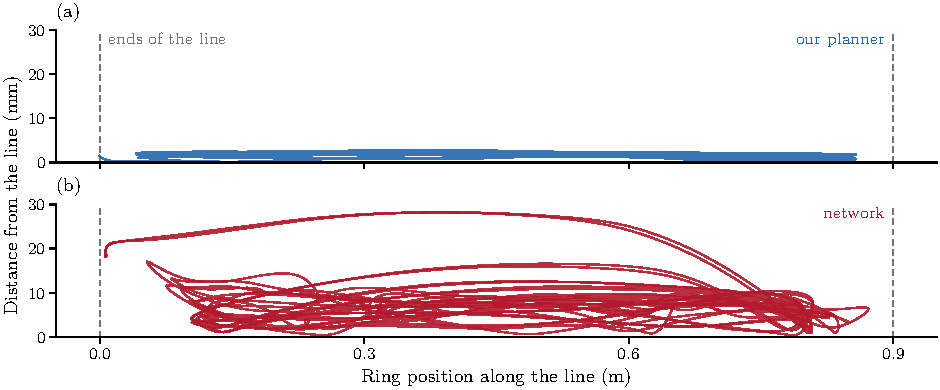
\includegraphics[width=\columnwidth]{figures/fig_c_line.pdf}
\caption{The 0.4\,m/s line in the twin: the ring's position along the line against the schedule, our planner and the
retuned network. The network runs about 1.1\,s late and turns short of each end.}
\label{fig:c_line}
\end{figure}

\begin{figure}[t]
\centering
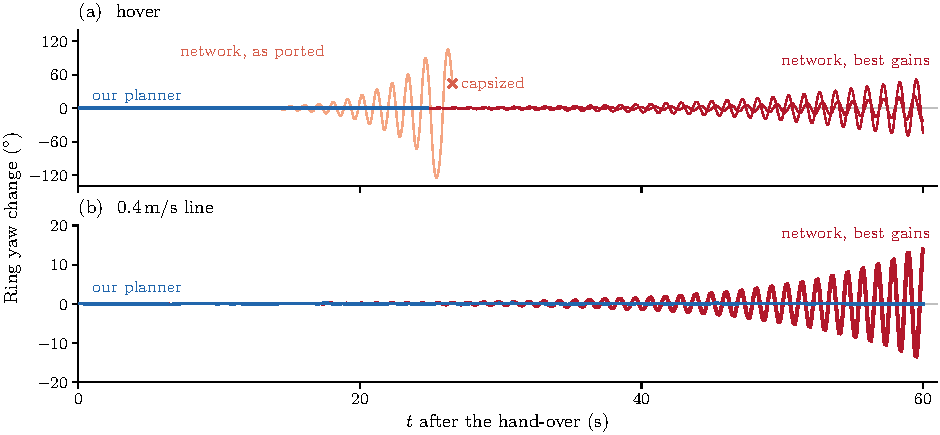
\includegraphics[width=\columnwidth]{figures/fig_c_yaw.pdf}
\caption{The ring's yaw after the hand-over in hover: the network as ported (it capsizes and the run aborts), the
retuned network (the yaw swings but the ring is held), and our planner.}
\label{fig:c_yaw}
\end{figure}

% 05_discussion.tex -- discussion and conclusion, draft 23 Oct 2026.
\section{Discussion}
\label{sec:discussion}

\paragraph{Rigid links in the twin, slack tethers on the rig}
The twin models every cable as a rigid link, which can push as well as pull and welds wherever its end lies. This
flatters the rejoin and also creates its own failure: on a T, the rejoiner's rigid link set the ring's pitch, so a
rising height reference lifted the ring's free side, and the height hold that cured it is a patch for the twin's
links. On the rig the tethers go slack, so that lift cannot arise, but the attach is harder: the magnet catches only on
contact, which is why the rig's attach is confirmed from motion capture before the newcomer is folded in. The rig's
release reaction, by contrast, needs no such caveat: it was measured on the rig, and the twin's release on longer
cables agreed in resize time and tilt.

\paragraph{Timing}
Every reconfiguration in Section~\ref{sec:results} is paced by detection and blending rather than by the solver: a
lost carrier is seen from its cable's stretch in 0.33--0.42\,s and the problem is resized within about 0.1\,s more,
and a rejoin's fold-in is blended over 10\,s. The solver sets the size of the team instead. At four carriers one SQP
iteration per tick flies as well as five in the twin's closed loop, but its plans are not converged on the rig's
flights, and at eight carriers only five iterations pass every bar (Section~\ref{sec:res_scale}). The eight-carrier
chain ran slower than real time, so it shows that the plan and the physics compose, not that the rig's laptop can fly
it.

\paragraph{The rim geometry}
The comparison with Quan et al.~\cite{quan2025swarm} turned on the attachment geometry rather than on the method's
code. With every cable at the ring's centre, the network held the ring's yaw to 0.1$^\circ$; with the cables on the
rim, as any payload with discrete attachment plates has them, the cables torque the ring in yaw and the network,
which has no yaw term, lets it swing (Section~\ref{sec:res_compare}). A planner that models each cable's attachment
point, as ours does, holds the yaw because the torque is in its model. For reconfiguration this matters doubly: a
release or a rejoin changes which plates carry the ring and so changes that torque.

\paragraph{Next on the rig}
The next rig flights test the attach of a newcomer on 1\,m cables, three carriers to four with a basket, with the
attach confirmed by motion capture before the fold-in; the four-carrier hover and paths on 1\,m cables; and the
planner's tick in flight with the speed-ups, which sets the real-time limit. The rejoin of a departed carrier, which
in the twin depends on the joint's weld, waits for a rig attach that has been shown repeatable.

\section{Conclusion}
\label{sec:conclusion}

We presented a planner that lets a team of quadrotors carry a cable-suspended ring through changes of its own
membership in flight. On the rig, an unannounced release of one of four carriers was detected in 0.42\,s, the team
was resized 0.09\,s later, and the ring tilted at most 6.5$^\circ$ before returning to its band in 1.8\,s. In the twin,
a departed carrier flew back to its own plate, welded within 1.5\,cm and was folded in with the ring tilting
1.3--3.4$^\circ$, and eight carriers took a larger ring down to four and back with a tilt peak of 3.35$^\circ$. Two SQP
iterations per tick converge for every fleet of up to four. Against a port of Quan et al.'s network method, our planner
held the ring's yaw where the network, lacking a yaw term for rim-attached cables, did not. The rig attach of a
newcomer on 1\,m cables is the next step \placeholder{result from 29 Oct}.


\bibliographystyle{IEEEtran}
\bibliography{refs}

\end{document}
